%使用xelatex编译
%版权所有,翻版必究
%本文件由程序自动生成,任何修改将被覆盖





%


\subsection{
qmake入门
}\label{s100310}


qmake类似于cmake,但qmake比cmake更加简洁清晰。
如果读者希望写一个跨平台的通用库的话,
或许cmake是比qmake更加优异的选择。
但读者明确是写一个特定的应用程序的话,
qmake就比cmake优秀的多。
qmake比cmake确实功能较少,
但从另一个角度,
qmake比cmake更加专注。
通过本节,
读者会发现只需要学习可怜的一点内容,
就可以使用qmake搭建出复杂的程序架构。
不过,本书毕竟是一门专门写Qt Quick的书,
不可能介绍qmake的每一个细节。

%%%%%%%%%%%%%%%%%%%%%%%%%%%%%%%%%%%%%%%%%%%%%%%%%%%%%%%%

\subsubsection{
使用qmake构建Hellow World!
}\label{ss000610}

读者新建一个目录\footnote{
本书所有目录都要求不包含空格和中文,以后不再赘述。
},
在此文件夹下新建一个“hellow\underline{\hspace{0.5em}}world.pro”文件,输入文件内容如
\lstlistingname\ \ref{f000002}。
在此文件夹下建立“main.cpp”文件,输入内容如
\lstlistingname\ \ref{f000003}。

%\begin{spacing}{1.0}
\begin{lstlisting}[label=f000002,
caption=GoodLuck,
title=\lstlistingname\ \thelstlisting
]
QT -= gui
QT -= core

CONFIG += console

CONFIG(debug,debug|release){
    TARGET = hellow_word_debug
}else{
    TARGET = hellow_word
}

TEMPLATE = app

win32-msvc*{
    QMAKE_CXXFLAGS += /std:c++latest
}else{
    CONFIG += c++17
}

SOURCES += $$PWD/main.cpp
DESTDIR =  $$PWD

DEFINES *= NUMBER=1
DEFINES *= HELLOW=\\\"Hellow\\\"
DEFINES += QT_DEPRECATED_WARNINGS
\end{lstlisting}          %抄录环境
%\end{spacing}

%\begin{spacing}{1.0}
\begin{lstlisting}[label=f000003,
caption=GoodLuck,
title=\lstlistingname\ \thelstlisting
]
#include <iostream>

int main(int , char **) {
    if constexpr(NUMBER) {
        std::cout << HELLOW " World! "
                  << std::endl;
    }
}
\end{lstlisting}          %抄录环境
%\end{spacing}


使用QtCreator打开“hellow\underline{\hspace{0.5em}}world.pro”,
运行此项目。

现在来分析一下\lstlistingname\ \ref{f000002}:
\begin{itemize}
\item 第1\~{}2行表示不使用Qt库;
\item 第4行表示这是一个控制台应用程序;
\item 第6\~{}10行表示在debug模式下输出目标名称是“hellow\underline{\hspace{0.5em}}world\underline{\hspace{0.5em}}debug”,
在release模式下输出目标名称是“hellow\underline{\hspace{0.5em}}world”;
\item 第12行表示输出的是一个应用程序;
\item 第14\~{}18行表示使用C++17标准;
\item 第20行将“main.cpp”加入编译过程;
\item 第21行规定输出目录就是当前“pro”文件所在目录;
\item 第23行定义了一个叫“NUMBER”的宏,宏的值是一个数字;
\item 第24行定义了一个叫“HELLOW”的宏,宏的值是一个字符串;
\item 第25行定义了一个叫“QT\underline{\hspace{0.5em}}DEPRECATED\underline{\hspace{0.5em}}WARNINGS”的宏,这个宏没有定义值;
\end{itemize}

不难发现qmake的语法十分简单:
\begin{itemize}
\item “=”代表赋值;
\item “+=”代表向变量中增加元素;
\item “-=”代表从变量中删除元素;
\item “*=”代表如果变量中不存在则加入元素否则忽略;
\item “\~{}=”代表替换变量中的值;
\item “\$\$”代表当qmake运行时,变量的字面值;
\item “\$”代表当qmake生成Makefile后,变量的字面值;
\item “\#”代表注释;
\item “SOURCES”代表需要编译的C/C++源代码变量;
\item “HEADERS”代表C/C++头文件变量;
\item “DEFINES”代表C/C++宏变量;
\item “TARGET”代表输出对象名称;
\item “CONFIG”用来加入和检查Qt中预定义的编译选项;
\item “QMAKE\underline{\hspace{0.5em}}CXXFLAGS”代表qmake生成Makefile时需要加入的编译器参数;
\item “TEMPLATE”决定此项目的模板类型,本案例是使用应用程序模板“app”,
顾名思义此模板的目标是生成应用程序。后续章节会介绍更多模板;
\end{itemize}

第6\~{}10行和14\~{}18虽然写法不同,实际上都是检查“CONFIG”中是否定义了特定项。
读者可以尝试一下向文件“hellow\underline{\hspace{0.5em}}world.pro”文件最后
加入\lstlistingname\ \ref{f00000d},
分别去掉\lstlistingname\ \ref{f00000d}第一行和
保留第一行,
观察qtcreator的“概要信息”输出什么。
%\begin{spacing}{1.0}
\begin{lstlisting}[label=f00000d,
caption=GoodLuck,
title=\lstlistingname\ \thelstlisting
]
CONFIG += mydebug
mydebug{
    message("find my debug")
}else{
    message("can not find my debug")
}
\end{lstlisting}          %抄录环境
%\end{spacing}




%
% 
%%%%%%%%%%%%%%%%%%%%%%%%%%%%%%%%%%%%%%%%%%%%%%%%%%%%%%

\subsubsection{
使用qmake创建动态链接库
}\label{ss000710}


绝大多数项目的项目结构都很复杂,从这一节开始读者要开始接受这一事实。
本节示例的项目结构如\treeindexnumbernameone\ \ref{d000001}
所示。

%\begin{spacing}{1.0}
\refstepcounter{treeindexnumber}\label{d000001}    %增加目录树编号
\begin{lstlisting}[caption=GoodLuck,
numbers=none,
title=\treeindexnumbernameone \thetreeindexnumber
]
.
├── import_library.pro
├── test_library
│   ├── import_test_library.pri
│   ├── TestLibrary.cpp
│   ├── TestLibrary.hpp
│   └── test_library.pro
└── the_app
    ├── main.cpp
    └── the_app.pro
\end{lstlisting}          %抄录环境
%\end{spacing}


先来看看“import\underline{\hspace{0.5em}}library.pro”文件,
如\lstlistingname\ \ref{f000010}所示。

此文件启用了一个新的模版,“subdirs”。

“subdirs”模版可以将一系列孤立的工程组织起来\footnote{
最好不要嵌套引用subdirs,某些IDE并不支持。
},
并要求它们按照一定先后顺序编译。
比如本节采用的“CONFIG += ordered”就要求项目按照定义顺序编译。

%\begin{spacing}{1.0}
\begin{lstlisting}[label=f000010,
caption=GoodLuck,
title=\lstlistingname\ \thelstlisting
]
#import_library.pro
TEMPLATE = subdirs

CONFIG += ordered

test_library.file = $$PWD/test_library/test_library.pro
SUBDIRS += test_library

the_app.file = $$PWD/the_app/the_app.pro
SUBDIRS += the_app
\end{lstlisting}          %抄录环境
%\end{spacing}


再来看看“the\underline{\hspace{0.5em}}app.pro”文件,
如\lstlistingname\ \ref{f000016} 所示。它采用了“app”模版。
比起上一节,它多了一些新的知识点。
\begin{itemize}
\item 第21\~{}23行更改了在非Windows平台下程序的链接参数,
它要求程序运行时将其所在目录加入动态库搜索路径;
\item 第28行将另一个文件引入此文件,它和C/C++的“\#include”工作原理一致;
\end{itemize}

%\begin{spacing}{1.0}
\begin{lstlisting}[label=f000016,
caption=GoodLuck,
title=\lstlistingname\ \thelstlisting
]
#the_app.pro
QT += gui
QT += core

CONFIG += console

CONFIG(debug,debug|release){
    TARGET = the_app_debug
}else{
    TARGET = the_app
}

TEMPLATE = app

win32-msvc*{
    QMAKE_CXXFLAGS += /std:c++latest
}else{
    CONFIG += c++17
}

!win32 {
    QMAKE_LFLAGS += -Wl,-rpath .
}

DESTDIR =  $$PWD/../bin

SOURCES += $$PWD/main.cpp
include($$PWD/../test_library/import_test_library.pri)
\end{lstlisting}          %抄录环境
%\end{spacing}


接下来是“import\underline{\hspace{0.5em}}test\underline{\hspace{0.5em}}library.pri”文件,
如\lstlistingname\ \ref{f000011} 所示。
它也引入了一些新的知识。
\begin{itemize}
\item 第2行使用“INCLUDEPATH”变量将当前目录加入C/C++包含路径搜索路径;
\item 第3\~{}7使用“LIBS”变量导入C/C++链接库,
“-L”后面是库所在路径,
“-l”后面紧跟库的名称;
\end{itemize}
%\begin{spacing}{1.0}
\begin{lstlisting}[label=f000011,
caption=GoodLuck,
title=\lstlistingname\ \thelstlisting
]
#import_test_library.pri
INCLUDEPATH += $$PWD
CONFIG(debug,debug|release){
    LIBS += -L$$PWD/../bin -ltest_libraryd
}else{
    LIBS += -L$$PWD/../bin -ltest_library
}
\end{lstlisting}          %抄录环境
%\end{spacing}


然后,我么来看一下如何使用qmake定义一个动态链接库。
一切与定义应用程序没什么不同,只是将
“TEMPLATE = app”改成了
“TEMPLATE = lib”,如\lstlistingname\ \ref{f000012} 第13行所示。

%\begin{spacing}{1.0}
\begin{lstlisting}[label=f000012,
caption=GoodLuck,
title=\lstlistingname\ \thelstlisting
]
#test_library.pro
QT += gui
QT += core

CONFIG += console

CONFIG(debug,debug|release){
    TARGET = test_libraryd
}else{
    TARGET = test_library
}

TEMPLATE = lib

win32-msvc*{
    QMAKE_CXXFLAGS += /std:c++latest
}else{
    CONFIG += c++17
}

!win32 {
    QMAKE_LFLAGS += -Wl,-rpath .
}

SOURCES += $$PWD/TestLibrary.cpp
HEADERS += $$PWD/TestLibrary.hpp

DESTDIR =  $$PWD/../bin
DEFINES *= D_TEST_LIBRARY
\end{lstlisting}          %抄录环境
%\end{spacing}
%test_library.pro


剩下的是
“TestLibrary.hpp”
(如\lstlistingname\ \ref{f000014}),
“TestLibrary.cpp”
(如\lstlistingname\ \ref{f000013})
和
“main.cpp”
(如\lstlistingname\ \ref{f000015})
。
都是标准C++,本书不赘述。
%\begin{spacing}{1.0}
\begin{lstlisting}[label=f000014,
caption=GoodLuck,
title=\lstlistingname\ \thelstlisting
]
/*TestLibrary.hpp*/
#pragma once

#include <QtCore/qglobal.h>

#ifndef D_TEST_LIBRARY
#define TEST_LIBRARY_EXPORT Q_DECL_IMPORT
#else
#define TEST_LIBRARY_EXPORT Q_DECL_EXPORT
#endif

class TEST_LIBRARY_EXPORT TestClass {
public:
    TestClass();
    ~TestClass();
    void foo();
};
\end{lstlisting}          %抄录环境
%\end{spacing}
%TestLibrary.hpp
%\begin{spacing}{1.0}
\begin{lstlisting}[label=f000013,
caption=GoodLuck,
title=\lstlistingname\ \thelstlisting
]
/*TestLibrary.cpp*/
#include "TestLibrary.hpp"
#include <iostream>

TestClass::TestClass() {
}

TestClass::~TestClass() {
}

void TestClass::foo() {
    std::cout << __func__ << std::endl;
}
\end{lstlisting}          %抄录环境
%\end{spacing}
%TestLibrary.cpp
%\begin{spacing}{1.0}
\begin{lstlisting}[label=f000015,
caption=GoodLuck,
title=\lstlistingname\ \thelstlisting
]
/*main.cpp*/
#include <TestLibrary.hpp>

int main(int, char **) {
    TestClass varClass;
    varClass.foo();
    return 0;
}
\end{lstlisting}          %抄录环境
%\end{spacing}
%main.cpp


%%%%%%%%%%%%%%%%%%%%%%%%%%%%%%%%%%%%%%%%%%%%%%%%%%%%%%%%

\subsubsection{
qmake高级用法
}\label{ss000810}


qmake远比读者想象的要复杂的多,
本节向读者展示一些常见功能如何使用qmake实现。


\begin{figure}[ht] %浮动体 here and top ...
\centering %中心对齐
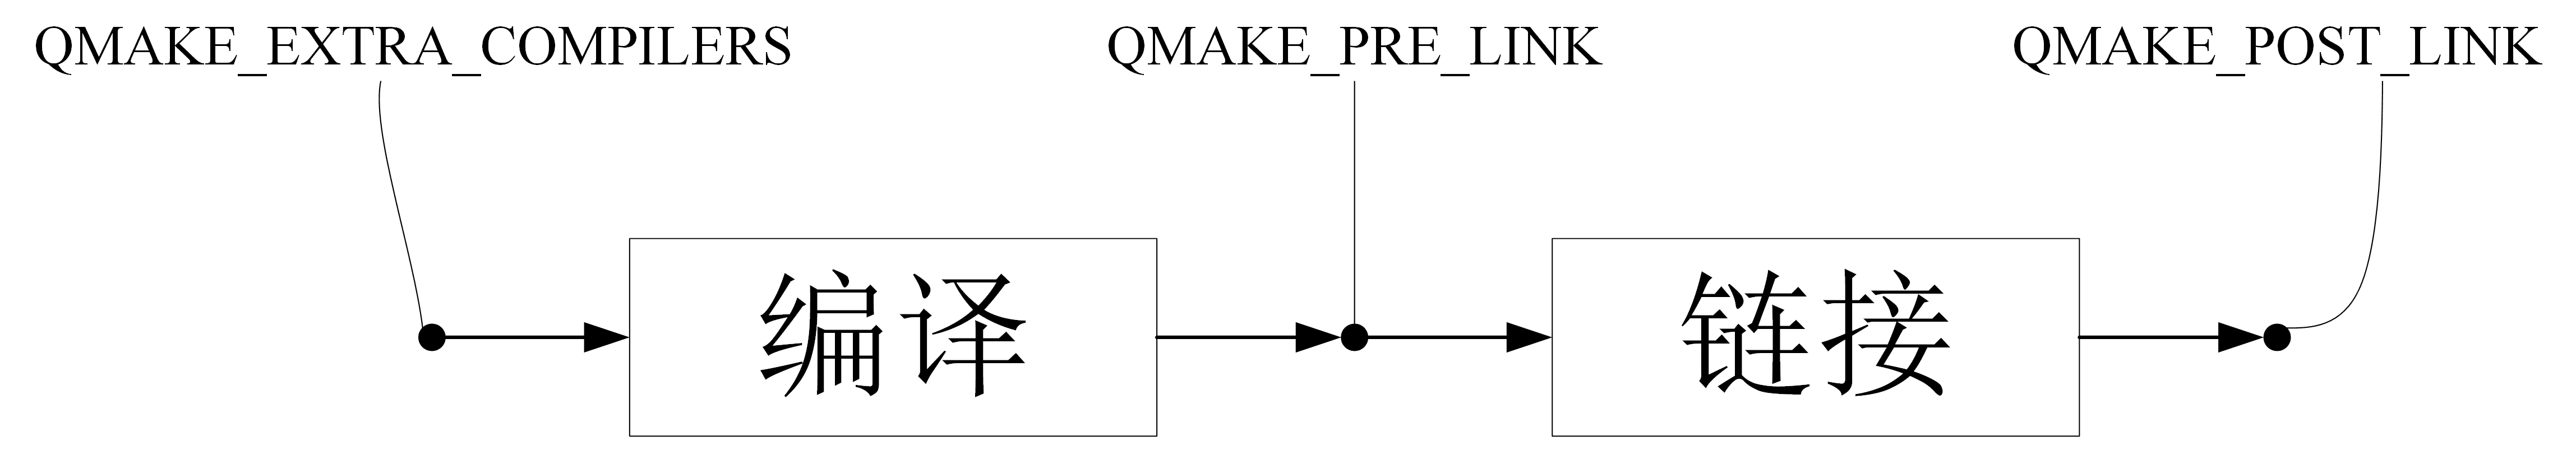
\includegraphics[width=\textwidth]{chapter01/images/advance_use_qmake.png} %图片路径
\caption{qmake对C/C++编译链接过程控制点} %标题
\label{p000002} %索引
\end{figure}


如\figurename\ \ref{p000002}
一个C/C++程序编译至少可以抽象出三个节点,
源代码编译前,
链接前以及链接后。
这三个时刻分别对应于qmake变量:
QMAKE\underline{\hspace{0.5em}}EXTRA\underline{\hspace{0.5em}}COMPILERS,
QMAKE\underline{\hspace{0.5em}}PRE\underline{\hspace{0.5em}}LINK以及
QMAKE\underline{\hspace{0.5em}}POST\underline{\hspace{0.5em}}LINK。

使用这三个控制变量,用户可以在这三个时刻执行自定义命令。

本节代码树
如\treeindexnumbernameone\ \ref{d000000}所示,
“advance\underline{\hspace{0.5em}}use\underline{\hspace{0.5em}}qmake.pro”文件
如\lstlistingname\ \ref{f000004}所示。

%\begin{spacing}{1.0}
\refstepcounter{treeindexnumber}\label{d000000}    %增加目录树编号
\begin{lstlisting}[caption=GoodLuck,
numbers=none,
title=\treeindexnumbernameone \thetreeindexnumber
]
.
├── advance_use_qmake.pro
├── after_run
│   ├── after_run.pro
│   └── main.cpp
├── before_run
│   ├── before_run.pro
│   └── main.cpp
├── new_moc
│   ├── main.cpp
│   └── new_moc.pro
└── the_run
    ├── main.cpp
    ├── test1.hpp
    ├── test2.hpp
    └── the_run.pro
\end{lstlisting}          %抄录环境
%\end{spacing}
 %tree.txt

%\begin{spacing}{1.0}
\begin{lstlisting}[label=f000004,
caption=GoodLuck,
title=\lstlistingname\ \thelstlisting
]
#advance_use_qmake.pro
TEMPLATE = subdirs

CONFIG += ordered

new_moc.file = $$PWD/new_moc/new_moc.pro
SUBDIRS += new_moc

before_run.file = $$PWD/before_run/before_run.pro
SUBDIRS += before_run

after_run.file = $$PWD/after_run/after_run.pro
SUBDIRS += after_run

the_run.file = $$PWD/the_run/the_run.pro
SUBDIRS += the_run
\end{lstlisting}          %抄录环境
%\end{spacing}
 %advance_use_qmake.pro

本案例向读者展示:
\begin{enumerate}
\item 在编译开始前,qmake调用“程序new\underline{\hspace{0.5em}}moc”自动生成cpp文件并加入编译过程;
\item 在连接前qmake调用“程序before\underline{\hspace{0.5em}}run”,“程序before\underline{\hspace{0.5em}}run”
向“the\underline{\hspace{0.5em}}run文件夹”下建立一个“before\underline{\hspace{0.5em}}run.txt文件”;
\item 在连接完成后qmake调用“程序after\underline{\hspace{0.5em}}run”,“程序after\underline{\hspace{0.5em}}run”
向“the\underline{\hspace{0.5em}}run”文件夹下建立一个“after\underline{\hspace{0.5em}}run.txt文件”;
\end{enumerate}



%\begin{spacing}{1.0}
\begin{lstlisting}[label=f000005,
caption=GoodLuck,
title=\lstlistingname\ \thelstlisting
]
#the_run.pro
QT -= gui
QT -= core

CONFIG += console

CONFIG(debug,debug|release){
    TARGET = the_run_debug
}else{
    TARGET = the_run
}

TEMPLATE = app

win32-msvc*{
    QMAKE_CXXFLAGS += /std:c++latest
}else{
    CONFIG += c++17
    LIBS += -lstdc++fs
}

SOURCES += $$PWD/main.cpp
DESTDIR =  $$PWD/../bin

DEFINES += QT_DEPRECATED_WARNINGS

#when before build new_moc will call ...
new_moc.dependency_type = TYPE_C
new_moc.variable_out =    SOURCES
new_moc.output  = moc_new_${QMAKE_FILE_BASE}.cpp
CONFIG(debug,debug|release){
new_moc.commands = \
$${DESTDIR}/new_moc_debug ${QMAKE_FILE_NAME} ${QMAKE_FILE_OUT}
}else{
new_moc.commands = \
$${DESTDIR}/new_moc ${QMAKE_FILE_NAME} ${QMAKE_FILE_OUT}
}
NEW_MOC_HEADERS = test2.hpp test1.hpp
new_moc.input = NEW_MOC_HEADERS
QMAKE_EXTRA_COMPILERS += new_moc
export(QMAKE_EXTRA_COMPILERS)

#when link started before_run will call ...
CONFIG(debug,debug|release){
    QMAKE_PRE_LINK += $${DESTDIR}/before_run_debug $$PWD
}else{
    QMAKE_PRE_LINK += $${DESTDIR}/before_run $$PWD
}
export(QMAKE_PRE_LINK)

#when link finished after_run will call ...
CONFIG(debug,debug|release){
    QMAKE_POST_LINK += $${DESTDIR}/after_run_debug $$PWD
}else{
    QMAKE_POST_LINK += $${DESTDIR}/after_run $$PWD
}
export(QMAKE_POST_LINK)
\end{lstlisting}          %抄录环境
%\end{spacing}
 %the_run.pro
%\begin{spacing}{1.0}
\begin{lstlisting}[label=f00000a,
caption=GoodLuck,
title=\lstlistingname\ \thelstlisting
]
/*main.cpp*/
#if __has_include(<filesystem>)
#include <filesystem>
namespace fs = std::filesystem;
#else
#include <experimental/filesystem>
namespace fs = std::experimental::filesystem;
#endif
#include <iostream>

int main(int, char **) {
    std::cout << "the_run" << std::endl;
    return 0;
}
\end{lstlisting}          %抄录环境
%\end{spacing}
 %the_run/main.cpp
%\begin{spacing}{1.0}
\begin{lstlisting}[label=f000006,
caption=GoodLuck,
title=\lstlistingname\ \thelstlisting
]
#after_run.pro
QT -= gui
QT -= core

CONFIG += console

CONFIG(debug,debug|release){
    TARGET = after_run_debug
}else{
    TARGET = after_run
}

TEMPLATE = app

win32-msvc*{
    QMAKE_CXXFLAGS += /std:c++latest
}else{
    CONFIG += c++17
    LIBS += -lstdc++fs
}

SOURCES += $$PWD/main.cpp
DESTDIR =  $$PWD/../bin

DEFINES += QT_DEPRECATED_WARNINGS
\end{lstlisting}          %抄录环境
%\end{spacing}
 %after_run.pro
%\begin{spacing}{1.0}
\begin{lstlisting}[label=f000007,
caption=GoodLuck,
title=\lstlistingname\ \thelstlisting
]
/*main.cpp*/
#if __has_include(<filesystem>)
#include <filesystem>
namespace fs = std::filesystem;
#else
#include <experimental/filesystem>
namespace fs = std::experimental::filesystem;
#endif

#include <iostream>
#include <fstream>
#include <chrono>

class OStream final : public std::ofstream {
    using Super = std::ofstream;
public:
    template<typename T,
        typename = std::enable_if_t<
        std::is_constructible_v<Super, T && > > >
        inline OStream(T && arg) :
        Super(std::forward<T>(arg)) {
    }
    template<typename T,
        typename = void,
        typename = std::enable_if_t<
        !std::is_constructible_v<Super, T && > > >
        inline OStream(T && arg) :
        Super(std::forward<T>(arg).string()) {
    }
};

/* 在特定文件夹下建立一个after_run.txt
 * 并输出程序运行时时间戳 */
int main(int argc, char ** argv) {
    std::cout << "after_run : "
        << argc << std::endl;
    if (argc < 2) {
        return -1;
    }
    fs::path varPath{ argv[1] };
    OStream stream{ varPath / "after_run.txt" };
    stream << std::chrono::
        high_resolution_clock::now()
        .time_since_epoch().count();
    stream << std::endl;
    return 0;
}
\end{lstlisting}          %抄录环境
%\end{spacing}
 %after_run/main.cpp
%\begin{spacing}{1.0}
\begin{lstlisting}[label=f000008,
caption=GoodLuck,
title=\lstlistingname\ \thelstlisting
]
#before_run.pro
QT -= gui
QT -= core

CONFIG += console

CONFIG(debug,debug|release){
    TARGET = before_run_debug
}else{
    TARGET = before_run
}

TEMPLATE = app

win32-msvc*{
    QMAKE_CXXFLAGS += /std:c++latest
}else{
    CONFIG += c++17
    LIBS += -lstdc++fs
}

SOURCES += $$PWD/main.cpp
DESTDIR =  $$PWD/../bin

DEFINES += QT_DEPRECATED_WARNINGS
\end{lstlisting}          %抄录环境
%\end{spacing}
 %before_run.pro
%\begin{spacing}{1.0}
\begin{lstlisting}[label=f000009,
caption=GoodLuck,
title=\lstlistingname\ \thelstlisting
]
/*main.cpp*/
#if __has_include(<filesystem>)
#include <filesystem>
namespace fs = std::filesystem;
#else
#include <experimental/filesystem>
namespace fs = std::experimental::filesystem;
#endif

#include <iostream>
#include <fstream>
#include <chrono>

class OStream final : public std::ofstream {
    using Super = std::ofstream;
public:
    template<typename T,
        typename = std::enable_if_t<
        std::is_constructible_v<Super, T && > > >
        inline OStream(T && arg) :
        Super(std::forward<T>(arg)) {
    }
    template<typename T,
        typename = void,
        typename = std::enable_if_t<
        !std::is_constructible_v<Super, T && > > >
        inline OStream(T && arg) :
        Super(std::forward<T>(arg).string()) {
    }
};

/* 在特定文件夹下建立一个before_run.txt
 * 并输出程序运行时时间戳 */
int main(int argc, char ** argv) {
    std::cout << "before_run : "
        << argc << std::endl;
    if (argc < 2) {
        return -1;
    }
    fs::path varPath{ argv[1] };
    OStream stream{ varPath / "before_run.txt" };
    stream << std::chrono::
        high_resolution_clock::now()
        .time_since_epoch().count();
    stream << std::endl;
    return 0;
}
\end{lstlisting}          %抄录环境
%\end{spacing}
 %before_run/main.cpp
%\begin{spacing}{1.0}
\begin{lstlisting}[label=f00000b,
caption=GoodLuck,
title=\lstlistingname\ \thelstlisting
]
#new_moc.pro
QT -= gui
QT -= core

CONFIG += console

CONFIG(debug,debug|release){
    TARGET = new_moc_debug
}else{
    TARGET = new_moc
}

TEMPLATE = app

win32-msvc*{
    QMAKE_CXXFLAGS += /std:c++latest
}else{
    CONFIG += c++17
    LIBS += -lstdc++fs
}

SOURCES += $$PWD/main.cpp
DESTDIR =  $$PWD/../bin

DEFINES += QT_DEPRECATED_WARNINGS
\end{lstlisting}          %抄录环境
%\end{spacing}
 %new_moc.pro
%\begin{spacing}{1.0}
\begin{lstlisting}[label=f00000c,
caption=GoodLuck,
title=\lstlistingname\ \thelstlisting
]
/*main.cpp*/
#include <iostream>
#include <fstream>

#if __has_include(<filesystem>)
#include <filesystem>
namespace fs = std::filesystem;
#else
#include <experimental/filesystem>
namespace fs = std::experimental::filesystem;
#endif

/*生成一个用于测试的.cpp,用于在控制台输出“Good Luck!”*/
int main(int argc, char ** argv) {
    std::cout << "new_moc : "
        << argc << std::endl;
    if (argc < 3) {
        return -1;
    }
    std::ifstream varInput{ argv[1] };
    std::ofstream varOutput{ argv[2] };
    varOutput << "/*****************************/";
    varOutput << std::endl;
    varOutput << "#include \"";
    varOutput << argv[1];
    varOutput << "\"";
    varOutput << std::endl;
    varOutput << u8R"(inline static int a = [](){
               std::cout << "Good Luck!" <<std::endl;
               return 12;
               }() ; )";
    varOutput << std::endl;
    return 0;
}
\end{lstlisting}          %抄录环境
%\end{spacing}
 %new_moc/main.cpp

%%%%%%%%%%%%%%%%%%%%%%%%%%%%%%%%%%%%%%%%%%%%%%%%%%%%%%%%

\subsubsection{
qmake杂项
}\label{ss000910}










%使用xelatex编译
%版权所有,翻版必究
%本文件由程序自动生成,任何修改将被覆盖



